\documentclass[11pt]{article}

\usepackage[review]{acl}

\usepackage{times}
\usepackage{latexsym}
\usepackage[T1]{fontenc}
\usepackage[utf8]{inputenc}
\usepackage{microtype}
\usepackage{inconsolata}
\usepackage{graphicx}
\usepackage{booktabs}

\title{Non-Exchangeability in KV-Cache Relay: From Fixed Pipelines to Recursive, Model-Driven Delegation}

\author{Anonymous ACL submission}

\begin{document}
\maketitle

\begin{abstract}
Multi-agent LLM systems increasingly relay key-value (KV) cache between
agents as a communication mechanism, implicitly treating the cache as a
transferable representation of state. Whether a receiving agent can treat
a relayed cache as interchangeable, rather than specifically tied to the
content that produced it, is rarely tested directly. We test it with a
causal intervention: at the point where one agent's KV cache would
normally be relayed to the next, we substitute it with (i) the correct,
real cache, (ii) an all-zero cache, (iii) a moment-matched random cache
(same per-tensor mean and standard deviation, no real structure), and
(iv) a real cache generated from a different, unrelated question. We
call a relayed cache non-exchangeable, in the empirical sense this paper
uses throughout, if substituting a mismatched but real cache measurably
changes downstream behavior relative to the correct cache, even though
the substitute has identical shape, dtype, and comparable statistics. We
apply this test across three structurally different multi-agent
topologies on Qwen2.5-7B-Instruct and HotpotQA: a fixed sequential
three-agent pipeline, a static fan-in decomposition, and a dynamic,
model-driven delegation loop built in the style of Recursive Language
Models (RLMs) \citep{rlm2026}, where the model itself writes and runs
code to decide what to delegate and when. In every topology we evaluate,
correct content outperforms mismatched real content, which outperforms
zeroed or random content, and the comparisons reach statistical
significance in each case; the fan-in topology gives the cleanest and
most decisive version of this result we observe. On a second model
family, Mistral-7B-Instruct-v0.3, the same ordering holds, though
layer-selection configurations show an attenuated pattern tied to that
configuration's own degraded baseline on this model, not to a loss of
content-dependence. On a third model, Qwen3-8B, we find the limit of the
claim rather than hiding it: random substitution still collapses
accuracy, but real content is not statistically distinguishable from
zeroed or mismatched content, indicating that content-dependence itself,
not only its magnitude, varies by architecture. We then turn to what
this implies for KV-cache compression and transformation, evaluating
five published or adapted techniques under this lens: uniform 8-bit
quantization preserves accuracy at no measurable cost; naive uniform
4-bit quantization collapses to incoherent output; a rotation-based
4-bit scheme fails for a diagnosable reason, disrupting the
position-dependent structure rotary position embeddings (RoPE) impose on
cached keys; a KIVI-inspired per-channel fix for keys resolves this,
reaching 3.96x compression at accuracy statistically indistinguishable
from our strongest layer-selection configuration (McNemar $p=0.86$); and
an anchor-based offset-correction mechanism adapted from KVCOMM
\citep{kvcomm2025} fails outright. Throughout, we report paired
significance tests and bootstrap confidence intervals, and we are
explicit about where our evidence is strongest (the fan-in topology, the
cross-architecture Qwen3-8B exception) and where it remains open (the
model-driven topology's KV-versus-text accuracy comparison, and a
single-GPU evaluation whose compression ratios do not constitute a
measured network-latency speedup).
\end{abstract}

\section{Introduction}

Multi-agent LLM systems need some way for one agent's work to reach the
next: a decoded text handoff, a shared latent representation, or,
increasingly, a directly relayed key-value (KV) cache. Relaying KV cache
is attractive specifically because it can avoid re-encoding information
the receiving agent would otherwise have to reprocess from text. This
attractiveness rests on an assumption that is rarely stated and, to our
knowledge, never directly tested: that some dimension of the cache
(which transformer layer, which channel within a head, which question's
content) can be treated as generic or interchangeable for the purpose of
compression, reconstruction, or reuse.

The question this paper asks is simple to state and, as far as we are
aware, has not been answered directly: can a KV cache produced for one
piece of content be treated as an interchangeable communication artifact,
or does it remain specifically tied to the content that produced it? The
intuition behind a causal test of this question is direct. If a relayed
cache merely carries generic, transferable state, replacing it with
another valid cache (same shape, same model, same rough statistics)
should not systematically change downstream behavior. If instead the
cache is content-specific, a real cache generated from a \emph{different}
question should be measurably harmful relative to the correct one, even
though it is just as valid a cache tensor.

We operationalize this with an intervention ladder of four conditions,
substituted at the exact point a cache would normally be relayed: the
correct \textbf{real} cache; an all-\textbf{zeroed} cache; a
\textbf{moment-matched random} cache, which preserves each tensor's own
mean and standard deviation but no real structure; and a \textbf{mismatched}
cache, a real cache generated from a different, held-out question. The
first three conditions ask, respectively, whether the receiver needs this
cache at all, whether something with the same coarse statistics can
substitute for it, and (through mismatched) whether a real cache carries
specific, not merely generic, content. The mismatched condition is the
most informative of the four: it is not a corrupted or out-of-distribution
input in the way zeroing or randomizing is, it is exactly as valid a cache
as the real one, generated by the same model on real content. If mismatched
content still measurably underperforms the correct content, that is direct
causal evidence that the cache's \emph{identity}, not merely its presence
or its statistics, is what the receiver is using. We define a relayed cache
as \textbf{non-exchangeable}, in the operational sense this paper uses
throughout, when substituting a real but mismatched cache for the correct
one changes downstream behavior under this test. This is an empirical,
causal claim about the models, tasks, and topologies we evaluate, not a
claim that KV caches can never be exchanged under any architecture or
task; we use language such as ``our results indicate'' and ``under the
evaluated models and tasks'' throughout rather than claiming a universal
property of all KV caches.

We test this progressively across three structurally distinct multi-agent
topologies, each broadening what the previous one could not rule out.
First, within a fixed sequential three-agent (Reasoner, Verifier,
Finalizer) pipeline, the simplest setting in which the question can be
asked, we find the causal ordering real $>$ mismatched $>$ zeroed/random,
with every comparison statistically significant. Second, we test whether
this is an artifact of a single sequential handoff by building a static
fan-in decomposition, where an aggregator receives two parallel sources
rather than one sequential chain; this setting is structurally fixed by
design just as the sequential pipeline is, but distinct in how content
reaches the receiver, and gives the cleanest, most decisive version of the
result in our entire evaluation. Third, we test whether the ordering
survives when the multi-agent topology is no longer fixed in advance at
all: a dynamic, model-driven delegation loop built in the style of
Recursive Language Models (RLMs) \citep{rlm2026}, where the root model
itself writes and executes code to decide, turn by turn, what to delegate
to a sub-call and when, and we substitute real KV cache for RLM's own
decoded-text return channel at the sub-call boundary. The same ordering
holds there too, significantly, including on a comparison final-answer
accuracy alone cannot resolve but a complementary behavioral signal, how
often the model commits to an answer within its turn budget, resolves
cleanly.

Having established this causal ordering, we turn to a practical
consequence: if relayed KV is genuinely content- and structure-specific,
compression or transformation schemes that implicitly assume some axis of
the cache is interchangeable (which layer, which channel, which position)
should be expected to fail in proportion to how much they rely on that
assumption, independent of whether they preserve coarse tensor statistics.
We test this directly on five published or adapted KV-relay efficiency
techniques within our fixed pipeline, and find exactly this pattern: a
cross-agent offset-correction method \citep{kvcomm2025} fails because it
assumes a deviation observed for one question transfers to another; a
rotation-based quantization scheme \citep{turboquant2026,polarquant2026}
fails specifically on key vectors because it assumes head dimensions are
interchangeable, disrupting the position-dependent structure RoPE
imposes on them; a per-channel quantization fix \citep{kivi2024} resolves
this by respecting that structure instead; and layer-selection's accuracy
cost turns out to be architecture-dependent in a way a calibration
procedure's own confidence does not predict, and misdirects on, which
model is safe to compress.

This paper makes three contributions.

\begin{itemize}
\item \textbf{Causal evidence for content-dependent KV relay.} We
systematically substitute relayed KV caches with zeroed, moment-matched
random, and mismatched real content, and show with paired statistical
tests that real content produces measurably different, and better,
downstream behavior than any of the three alternatives in a fixed
sequential pipeline, establishing the content-dependence claim this
paper builds on directly rather than assuming it.

\item \textbf{Generalization across communication topologies, including
one the model constructs for itself.} We show the same causal ordering
holds not only in the fixed sequential pipeline but in a static fan-in
decomposition (our cleanest result) and in a dynamic, model-driven
delegation loop in the style of RLMs, where the topology itself is not
fixed in advance by a system designer. We also show, rather than hide,
that this generalization has a limit: on Qwen3-8B, the same audit finds
content-dependence itself is not statistically distinguishable for two
of the three comparisons, indicating the phenomenon is
architecture-dependent.

\item \textbf{Implications for KV-cache transformation and compression.}
Building on the causal finding, we evaluate five techniques for reducing
or transforming relayed KV and show their effects vary sharply: one
quantization scheme is free, one collapses catastrophically, a
rotation-based fix fails for a diagnosable, RoPE-specific reason, a
per-channel fix resolves it at genuine compression, and an offset-
correction mechanism fails outright. We report these as consequences of
non-exchangeability rather than as a parallel, independent set of
results.
\end{itemize}

\section{Related Work}
\label{sec:related}

\paragraph{Cross-agent KV-cache relay.} Relaying key-value cache instead
of decoded text between agents has been proposed to avoid redundant
prefill computation. KVCOMM \citep{kvcomm2025} introduced an anchor-based
framework that estimates and corrects KV-cache offset drift when reusing
cache across different prefix contexts, reporting over 70\% cache reuse
and up to 7.8x prefill speedup on retrieval-augmented generation, math
reasoning, and coding tasks. LatentMAS \citep{latentmas2026} extends this
to full latent-space collaboration, exchanging autoregressively generated
latent ``thoughts'' via KV-cache working memory rather than relaying
already-decoded text, reporting token savings and accuracy gains across
nine math, science, and code benchmarks. We differ from both by relaying
real, decoded reasoning text through a fixed sequential three-agent chain
(Reasoner, Verifier, Finalizer) rather than offset-corrected reuse or
latent thought generation, and by evaluating on multi-hop QA
\citep{hotpotqa2018}, which neither tested on.

\paragraph{Compressing the relayed cache.} Reducing what must be
transmitted between agents is a natural complement to relay itself. We
adopt two families of technique: layer-wise selection, which drops
calibration-identified low-importance transformer layers before
transmission and reconstructs them at the receiver via \texttt{zeros},
\texttt{nearest}, or \texttt{interpolate}, and per-head quantization,
which reduces numeric precision. A third reconstruction strategy,
Orthogonal Backfill \citep{orthobackfill2026}, injects a low-rank residual
of discarded content orthogonal to what is retained rather than
substituting or discarding it outright; we considered but did not
implement it (see Limitations). KV-cache compression is also under active
industrial development: KVTC \citep{kvtc2026} applies media-compression-
style transform coding (PCA decorrelation, adaptive quantization, entropy
coding) for up to 20x compression, a third paradigm distinct from uniform
quantization (ours, KIVI) and rotation (TurboQuant/PolarQuant); NVIDIA's
kvpress library and TensorRT-LLM's reuse-aware cache confirm this is an
actively contested axis of real deployed systems, not a narrow academic
concern.

\paragraph{Rotation-based quantization interacts badly with RoPE-encoded
keys: a finding, not just an implementation note.} We initially
implemented a rotation-based quantization scheme in the style of
TurboQuant \citep{turboquant2026} and PolarQuant \citep{polarquant2026}
(two distinct papers sharing only two authors, not one work under two
names), applying a fixed orthonormal Hadamard rotation to both keys and
values before quantizing, to redistribute per-head outlier magnitude
(covering PolarQuant's rotate-then-quantize step, not TurboQuant's
separate QJL bias-correction term). On our real model this produced
severely out-of-distribution decoded output, not the graceful degradation
a generic rotation-based scheme predicts. We traced this to keys' rotary
position embeddings (RoPE): K is cached after RoPE is applied, which
mixes channel pairs by a position-dependent phase, and a second,
RoPE-agnostic rotation on top disrupts that structure rather than merely
redistributing outlier magnitude. An isolating ablation, rotating only V
and leaving K unrotated, reverted the failure to ordinary quantization-
noise degradation, confirming the interaction was with K specifically.
This is consistent with an established interaction in the KV-
quantization literature discussed next, and we report it as a diagnosed
negative result rather than an implementation detail (full diagnostic
examples in Appendix~\ref{app:rotation}).

\paragraph{RoPE-aware KV cache quantization.} A separate line of work
addresses exactly this interaction directly. KIVI \citep{kivi2024}
quantizes the key cache per-channel and the value cache per-token,
motivated by RoPE leaving channel-wise magnitude more consistent across
positions than uniform per-head ranges assume, rather than by rotating.
RotateKV \citep{rotatekv2025} instead applies rotation \emph{before} RoPE
via Pre-RoPE Grouped-Head Rotation, explicitly designed to avoid the
interaction we observed. KVQuant \citep{kvquant2024} and related work
similarly identify post-RoPE key quantization as harder than value
quantization for exactly this reason. We adopt a scoped, KIVI-inspired
fix (per-channel key quantization only, no group-wise windowing or
streaming residual buffer from the original method) and find it resolves
the collapse: from 0.0\%/0.0\% to 52.0\%/64.1\% F1 at $n=100$,
statistically indistinguishable from our strongest layer-selection
configuration (\texttt{D}; McNemar $p=0.86$) at higher compression (3.96x
versus \texttt{D}'s 3.82x, both relative to uncompressed relay) with no
calibration profile required. This is direct empirical confirmation, on
our pipeline and task, of what this literature identifies as the correct
axis for addressing the problem, rather than the rotation-based axis we
tried first. Whether KIVI's other asymmetric half (per-token value
quantization) adds anything on top is tested in Results.

\paragraph{Auditing whether KV reuse does what it claims.} A recent line
of work interrogates cross-agent KV or latent reuse critically rather
than only reporting end-task accuracy. ``When KV Cache Reuse Fails in
Multi-Agent Systems'' \citep{kvreusefails2026} shows reuse strategies
effective for generation agents can silently corrupt an LLM judge's
cross-candidate comparison even when end-task accuracy appears stable.
Cheng et al.\ \citep{latentcommpay2026} propose the specific intervention
we adopt: replacing relayed KV with mismatched, zeroed, or moment-
matched-random substitutes to test whether accuracy is causally
attributable to the specific transmitted content rather than to the
receiver simply having a non-empty cache. We build directly on this
causal intervention framework rather than claim it as our own invention,
and extend the analysis along two axes neither Cheng et al.\ nor the
other paper above tests: cross-architecture generalization, treating
whether the same technique, faithfully reproduced, transfers to a
different model family as itself a target of audit; and, more centrally
to this paper, generalization across communication topologies, testing
whether the same audit still finds real causal content-dependence once
the multi-agent structure itself is no longer fixed in advance. Notably,
Cheng et al.'s own headline finding is that content-specificity is
\emph{system}-dependent (ceiling on LatentMAS, partial on KVComm, no
detected advantage on C2C), holding audit methodology fixed and varying
which published relay system is tested. Our own extensions to Qwen3-8B
and, in a secondary check, to the C2C bridge itself independently arrive
at the same qualitative pattern, that content-specificity is not
universal, while holding audit methodology (and, in the Qwen3-8B case,
the relay mechanism) fixed and varying the model instead. Two independent
audits converging on ``it depends, and not on accuracy alone'' from
different varied axes is, we think, more informative than either result
read in isolation.

\paragraph{Model-driven delegation and recursive relay.} Recursive
Language Models \citep{rlm2026} let a root model decompose and delegate
via a live, sandboxed Python REPL rather than a topology the system
designer fixes in advance: the model decides what to send to a sub-call
and when, and reads the sub-call's answer back as a decoded-text REPL
variable it may or may not inspect before continuing. LatentMAS
\citep{latentmas2026} and CanonicalMerge \citep{canonicalmerge2026}, both
discussed above, relay something richer than text between agents, but
both over a topology fixed by the system designer: a sequential chain of
latent thoughts and a two-child fan-in merge, respectively, not one the
model constructs for itself turn by turn. CanonicalMerge in particular is
close to our own static fan-in topology: near-identical models
(Qwen3-1.7B/4B versus our Qwen2.5-7B-Instruct/Mistral-7B-Instruct-v0.3)
and a closely related task (HotpotQA bridge questions versus our full
distractor-setting HotpotQA), addressing a real methodological question
we do not, whether the order children are merged in biases the result,
but reporting only downstream accuracy, with no causal-intervention test
of whether the merged content is specifically, not just numerously,
necessary. We build a genuinely dynamic, model-driven delegation loop in
RLM's own style, substitute real KV cache for its text return channel at
the sub-call boundary, and apply the same causal-audit methodology used
throughout this paper to it. To our knowledge, no prior work (RLM's own
released implementation, LatentMAS, CanonicalMerge, or the causal-audit
literature discussed above) tests whether relayed content is causally
necessary once the delegation structure itself is no longer fixed by the
system designer.

\paragraph{Layer redundancy is not universal.} ``No Free Swap''
\citep{nofreeswap2026} finds that which transformer layers are
functionally interchangeable across Qwen3-8B, Llama-3.1-8B, and
Mistral-7B-v0.1 depends on the model and evaluation protocol rather than
being a fixed architectural property. This is consistent with our own
finding that a near-identical proportion of dropped layers costs
substantially more accuracy on Mistral-7B-Instruct-v0.3 than on
Qwen2.5-7B-Instruct, and offers one candidate mechanism for why.

\paragraph{Three 2026 papers anticipate pieces of this paper's argument.}
``Rethinking Layer Redundancy'' \citep{rethinkredundancy2026} argues
redundancy is a joint function of model and calibration objective, and
that a universal layer ranking may not exist, raising the question of
whether our cross-architecture gap is really about the model or about our
calibration ranking failing to transfer. We tested the most direct proxy:
whether the calibration signal's own confidence (the separation between
kept- and dropped-layer importance scores) predicts which model is safe
to compress. It does not, and fails in the wrong direction: Mistral's
tier separation (0.673) is larger, not smaller, than Qwen's (0.491),
despite Mistral being the more fragile model when that ranking is acted
upon. This is a direct empirical test of exactly the concern that paper
raises, and supports a stronger reading: not just that redundancy is
calibration-objective-dependent, but that the objective's own confidence
is not a reliable signal of when its ranking is safe to trust, consistent
with our broader claim that non-exchangeability is not visible from a
technique's internal signals.

AdaK \citep{adak2026} reports that adaptive KV-budget estimation
generalizes across Qwen3 (4B/8B) and Mistral-7B-Instruct-v0.2, the same
two architecture families this paper tests, not a third (Llama is not
among AdaK's evaluated models, though a superficial reading of the
abstract could suggest otherwise), which on its face looks like a
counterexample to our architecture-dependence claim. We do not believe it
is: AdaK estimates budget per-instance and per-model at inference time
rather than committing to a single calibration-time ranking applied
uniformly thereafter, so it never assumes a fixed, transferable ranking
is safe to act on. Read this way, AdaK's success is a positive instance
of our principle, not a counterexample; it works specifically because it
avoids the fixed-ranking assumption our own \texttt{D} configuration
makes. This is our reading of the mechanism, not something we verified
by reimplementing AdaK ourselves; a direct head-to-head comparison on our
own pipeline is noted in Limitations.

Finally, ``The Pitfalls of KV Cache Compression'' \citep{pitfallskv2026}
makes a general version of the point this paper investigates concretely:
that compression methods optimize for aggregate metrics while implicitly
equating token retention with functional preservation. Our contribution
is not the abstract observation but a causally grounded, cross-axis
demonstration of it within one system: the same failure pattern recurs
across three structurally distinct axes of KV-cache structure (depth,
position, content-identity) in a single pipeline, with the content-
identity axis validated causally via our audit rather than inferred from
compression metrics alone. We position this paper as the causal,
cross-axis synthesis these three papers each gesture toward from a
different angle.

\section{Method}
\label{sec:method}

\paragraph{Pipeline.} We study a sequential three-agent pipeline
(Reasoner, Verifier, Finalizer) answering HotpotQA \citep{hotpotqa2018}
(distractor configuration) questions, where each item bundles its own
ten candidate passages and requires no retrieval step; a GSM8K
\citep{gsm8k2021} confirmatory check in Results uses the same pipeline
structure. Agents share the same prompt structure and role definitions
across every configuration in this paper; the only thing that varies
between configurations is how one agent's output reaches the next. In
\texttt{text\_agent}, the Reasoner's decoded text is passed to the
Verifier as a literal string, which reads and reprocesses it from
scratch. In every KV-relay configuration (\texttt{A} through \texttt{E}),
the Reasoner's key-value cache, its internal representation of the
question, context, and its own generated reasoning, is passed directly
to the Verifier, which continues generation from that cache instead of
re-reading text. \texttt{single\_agent} is a no-relay control: one model
call, no intermediate agents at all. All KV-relay configurations share
identical prompts with \texttt{text\_agent}, so any accuracy or latency
delta between a KV configuration and \texttt{text\_agent} is attributable
to the relay mechanism itself, not to prompt differences.

\paragraph{Models.} We evaluate on Qwen2.5-7B-Instruct
\citep{qwen2p5_2024} (bf16) as our primary model, and, specifically to
test whether findings generalize across architecture rather than within
one model family, Mistral-7B-Instruct-v0.3 \citep{mistral7b2023} (bf16),
chosen for its architectural differences (distinct layer count, attention
head configuration, and tokenizer) at comparable parameter scale. Both
are decoder-only transformers using grouped-query attention and RoPE. A
third model, Qwen3-8B (Qwen Team, 2025, bf16), is evaluated on
configurations \texttt{A} and \texttt{D} only ($n=50$), specifically to
extend the architecture-dependence check and the tier-separation
comparison to a third data point, not to replicate the full causal-audit
suite. A fourth candidate, Phi-3.5-mini-instruct, was evaluated and
dropped after isolating a pre-existing LongRoPE limitation unrelated to
our pipeline (see Limitations).

\paragraph{Compression configurations.} \texttt{B\_int8}/\texttt{B\_int4}
apply uniform per-head min-max quantization to every transmitted layer's
key and value tensors (a fix to \texttt{B\_int4}'s originally catastrophic
failure is detailed in Results). \texttt{C} applies calibration-driven
layer selection, dropping transformer layers a per-model calibration pass
identifies as low-importance before transmission, reconstructing dropped
layers at the receiver via one of three strategies (\texttt{zeros},
\texttt{nearest}, \texttt{interpolate}). \texttt{D} combines layer
selection with adaptive per-layer-tier quantization (high-importance
layers at 8-bit, medium-importance at 4-bit). \texttt{E} adds an
anchor-based cross-agent offset-correction mechanism adapted from KVCOMM
(a negative result for this configuration, reported in Results).

\paragraph{RoPE-aware quantization fix for \texttt{B\_int4}.}
\texttt{B\_int4} (uniform 4-bit, no layer selection) initially collapsed
to 0.0\% accuracy, diagnosed as a quantization/RoPE interaction and
confirmed via two ablations (Related Work; full diagnostic detail in
Appendix~\ref{app:rotation}). Our fix (\texttt{B\_int4\_kivi}), inspired
by KIVI, quantizes keys per-channel (one numeric range per head
dimension, computed across positions) instead of per-head, leaving
values unchanged.

\paragraph{Statistical methodology.} For every headline comparison
between two configurations, we report exact (binomial-form) McNemar's
test on paired per-example correctness, appropriate because both
configurations are evaluated on the identical example set, and a paired
bootstrap 95\% confidence interval (10,000 resamples) for the difference
in mean token-F1. We additionally report Monte Carlo-estimated statistical
power at the current sample size for comparisons that do not reach
significance, so that ``not significant'' and ``confirmed no effect'' are
never conflated in our reporting.

\paragraph{Causal audit.} To test whether a configuration's accuracy
reflects the receiving agent using the specific transmitted content,
rather than merely having some non-empty cache to attend over, we
substitute the relayed KV cache with (i) an all-zero cache, (ii) a
moment-matched random cache (same per-tensor mean and standard deviation,
no real structure), and (iii) another, unrelated held-out question's real
cache at the same pipeline stage, sampled from a pool built from examples
never included in the scored evaluation set, so no scored question's
content can leak back to itself. We apply this to our three strongest
configurations (\texttt{A}, \texttt{B\_int8}, \texttt{D}).

We deliberately do not treat these three conditions as interchangeable
evidence for the same claim. Zero-ablation is a known-imperfect causal
baseline in the interpretability literature: it pushes activations off
the training distribution, which can produce large behavioral changes for
reasons unrelated to whether the zeroed content carried meaningful
information. We treat the moment-matched-random and mismatched-example
conditions, which preserve realistic activation statistics or substitute
another real, in-distribution cache, as the more informative evidence,
and zero-ablation as a supplementary sanity floor; if zeroing alone
diverges sharply from the other two, we attribute that to the out-of-
distribution effect rather than content-dependence. A fully rigorous
treatment of ``no difference'' would also use a pre-registered
equivalence margin rather than absence of significance under our paired
test; we did not have the budget to pre-register and power such a test,
and report significance and confidence-interval results with that
caveat.

\paragraph{Fan-in topology.} To test whether content-identity non-
exchangeability is an artifact of our sequential chain specifically, we
build a static fan-in decomposition: HotpotQA's ten candidate passages
are split across two independent child agents, each computing its own KV
cache over its half; the two caches are RoPE-position-shifted (reusing
the same primitive as our offset-correction baseline) and concatenated
before one aggregator attends over both and answers, so the aggregator
receives two parallel sources rather than one sequential handoff. The
causal audit substitutes every child's KV, not a single child while
leaving the other's real content available as an unaudited shortcut (an
early design bug we found and fixed; see Appendix~\ref{app:faninbug}),
matching the full-relay-corruption strength of the sequential pipeline's
own audit.

\paragraph{Dynamic, model-driven delegation (RLM+KV).} Our central
topology extension builds a real, sandboxed Python REPL loop in RLM's own
style \citep{rlm2026}: the root model writes and executes code turn by
turn, deciding for itself which passages to inspect directly and when to
delegate a sub-question to a child call, continuing until it calls a
terminal \texttt{final\_answer(...)}. We implement two sub-call return
channels to isolate the variable RLM itself does not test: \texttt{text},
matching RLM's own mechanism, decodes a sub-call's answer to text and
feeds it back as new tokens; \texttt{kv} instead RoPE-shifts and splices
the sub-call's own real KV cache directly onto the root's running cache,
so the root never observes the sub-call's answer as text at all. Both
conditions require the root to carry a real, continuously extended KV
cache across turns rather than re-tokenizing the full transcript each
turn, unlike RLM's own reference implementation, so that the two return
channels differ only in what is relayed, not in how the root's own
generation mechanism works. The causal audit substitutes a sub-call's
real KV with zeroed, random, or a held-out question's real content
immediately before the splice, identically to the two fixed topologies.
One structural difference from both fixed topologies is a genuine
limitation, not an oversight: the root retains direct sandboxed access to
the original passages independent of any sub-call, so corrupting a sub-
call's relayed KV does not remove all of the root's information the way
corrupting an entire relayed context does in the fixed topologies (see
Results and Limitations for how this shapes what the audit can and
cannot show).

We implement this ourselves directly on \texttt{transformers}
\citep{transformers2020} rather than on top of \texttt{dspy.RLM}, the
first-party DSPy implementation of RLM by one of the paper's own authors.
This is a structural necessity, not a preference: DSPy is built on
\texttt{litellm} and is, by design, a text-only, API-centric orchestration
layer; a sub-call through \texttt{dspy.RLM}'s own \texttt{llm\_query}
returns decoded text and nothing else, with no exposure anywhere in the
framework to a model's KV cache or other internal state. Our \texttt{kv}
return channel is not implementable on top of it. We verified this
directly against DSPy's own documentation rather than assume it from the
framework's general reputation before committing to a from-scratch
implementation.

\section{Results}
\label{sec:results}

We present results in the order the paper's argument is built. We first
establish, on the simplest topology, that relayed KV carries real,
content-specific information rather than merely being a non-empty cache
(Finding 1), and immediately surface where this finding's generalization
across architecture has a limit (Finding 2 and later, Qwen3-8B). We then
test whether the same causal ordering survives two structurally different
generalizations of the topology itself, a static fan-in decomposition
(Finding 4, our cleanest result) and a dynamic, model-driven delegation
loop (Finding 5). Only after this causal foundation do we turn to what it
implies for KV-cache compression and transformation (Findings 6 through
11).

\begin{figure}[t]
\centering
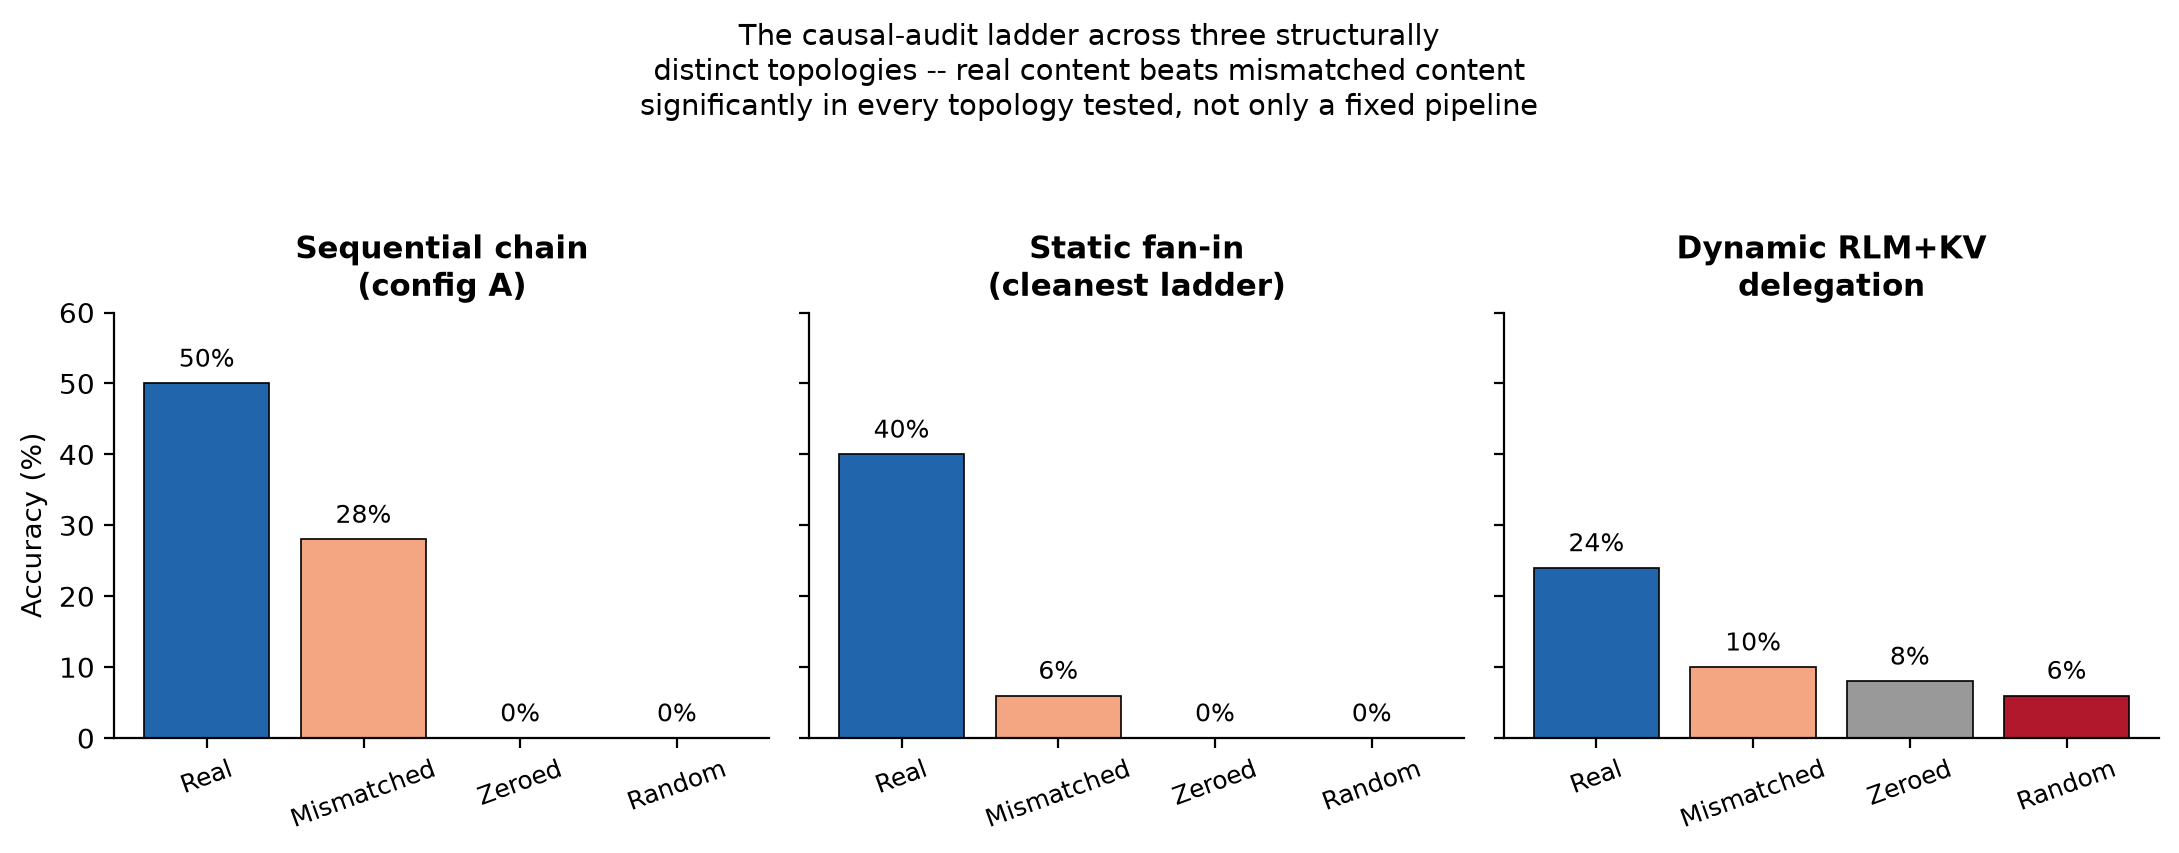
\includegraphics[width=\columnwidth]{figures/fig4_topology_ladder.png}
\caption{The causal-audit ladder across all three topologies tested in
this paper. Real content beats mismatched content, which beats
zeroed/random content, in every topology, including one the model
constructs for itself turn by turn, not only a fixed pipeline. The
recursive topology's non-zero zeroed/random floor is a real, discussed
scope difference (Section~\ref{sec:method}), not noise.}
\label{fig:topology_ladder}
\end{figure}

\paragraph{Finding 1 (headline): relayed KV demonstrably carries
specific, real content, not merely a non-empty cache.} We ran the causal
audit (Section~\ref{sec:method}) on \texttt{A} (uncompressed relay,
sequential chain), $n=50$: 50.0\%/64.0\% real versus zeroed/random both
0.0\%/0.0\% versus mismatched 28.0\%/37.1\%. Every pairwise comparison is
significant (real versus zeroed/random $p<0.0001$ each; real versus
mismatched $p=0.0127$; mismatched versus zeroed/random $p=0.0001$ each).
To our knowledge this is the first direct causal validation of this kind
for a sequential multi-agent KV-relay chain, and it underwrites every
compression result later in this paper: those results are only
meaningful claims about preserved information if the underlying relay
carries real content in the first place, which this finding establishes
directly rather than assuming. Qualitatively, mismatched's wrong answers
are coherent and grammatical, real linguistic structure attached to the
wrong question; zeroed produces garbled but recognizable English; and
random is more degraded still (code-fragment tokens, mixed-language
noise) despite matching real activation statistics. We read this as a
zero vector being a weak attention key that can be down-weighted, while
realistic random noise resembles genuine signal and actively misdirects
attention.

Table~\ref{tab:causal_audit_full} reports every subsequent extension of
this audit in one place: five relay configurations on Qwen2.5-7B-
Instruct/HotpotQA, five on Mistral-7B-Instruct-v0.3, two on Qwen3-8B, one
on GSM8K, and one each on the two topology extensions discussed below.
Across every Qwen2.5/HotpotQA configuration (\texttt{D}, \texttt{B\_int8},
\texttt{C}, \texttt{B\_int4\_kivi}), the same three-tier ordering
replicates, with real versus zeroed/random significant at $p<0.0001$ in
every case and real versus mismatched significant throughout
($p=0.0013$--$0.0192$); a single GSM8K \citep{gsm8k2021} confirmatory run
replicates it more decisively still ($p<0.0002$ throughout), showing the
claim is not an artifact of one task. Mismatched versus zeroed/random
across all these configurations lands at $p=0.0001$--$0.0005$, tighter
than \texttt{A}'s own $p=0.0001$.

% Consolidated causal-audit table -- draft for review before insertion into main.tex.
% Covers every real/zeroed/random/mismatched comparison currently spread
% across six "Finding 5, extended..." paragraphs, plus the new topology
% generalization rows (fan-in, RLM+KV) not yet in main.tex.

\begin{table*}[t]
\centering
\small
\begin{tabular}{llcccccc}
\toprule
\textbf{Config} & \textbf{Model / Task / Topology} & \textbf{Real} & \textbf{Zeroed} & \textbf{Random} & \textbf{Mismatched} & \textbf{$n$} \\
\midrule
\multicolumn{7}{l}{\emph{Qwen2.5-7B-Instruct, HotpotQA, sequential chain}} \\
A            & --                          & 50.0/64.0 & 0.0/0.0  & 0.0/0.0  & 28.0/37.1 & 50 \\
D            & --                          & 54.0/60.2 & 0.0/0.0  & 0.0/0.2  & 26.0/32.2 & 50 \\
B\_int8      & --                          & 54.0/68.0 & 0.0/0.0  & 0.0/0.0  & 24.0/34.4 & 50 \\
C            & --                          & 46.0/55.7 & 0.0/0.0  & 0.0/0.0  & 24.0/38.9 & 50 \\
B\_int4\_kivi& --                          & 50.0/61.7 & 0.0/0.0  & 0.0/0.0  & 28.0/34.7 & 50 \\
\midrule
\multicolumn{7}{l}{\emph{Generalization: model, task, and topology}} \\
A            & Mistral-7B-Instruct-v0.3    & 56.0/63.3 & 0.0/0.5  & 0.0/0.3  & 16.0/26.4 & 50 \\
C            & Mistral-7B-Instruct-v0.3    & 20.0/30.3 & 0.0/0.5  & 0.0/0.1  & 14.0/26.1 & 50 \\
D            & Mistral-7B-Instruct-v0.3    & 22.0/32.8 & 0.0/0.5  & 0.0/0.1  & 16.0/29.3 & 50 \\
B\_int8      & Mistral-7B-Instruct-v0.3    & 56.0/63.3 & 0.0/0.5  & 0.0/0.1  & 20.0/29.3 & 50 \\
B\_int4\_kivi& Mistral-7B-Instruct-v0.3    & 54.0/63.2 & 0.0/0.5  & 0.0/0.1  & 16.0/25.0 & 50 \\
A            & Qwen3-8B                    & 54.0/67.2 & 46.0/55.8& 0.0/0.0  & 64.0/74.8 & 50 \\
D            & Qwen3-8B                    & 56.0/71.2 & 46.0/55.8& 2.0/5.0  & 52.0/62.4 & 50 \\
A            & GSM8K (Qwen2.5)             & 90.0/---  & 0.0/---  & 2.0/---  & 28.0/---  & 50 \\
A            & 2WikiMultihopQA (Qwen2.5)   & 54.0/62.5 & 0.0/0.7  & 0.0/0.0  & 16.0/23.4 & 50 \\
kv (fan-in)  & Fan-in topology (Qwen2.5)   & 40.0/53.0 & 0.0/0.8  & 0.0/0.0  & 6.0/12.0  & 50 \\
kv (RLM+KV)  & Dynamic delegation (Qwen2.5)& 24.0/32.3 & 8.0/11.2 & 6.0/9.2  & 10.0/15.5 & 50 \\
\bottomrule
\end{tabular}
\caption{Every real/zeroed/random/mismatched causal-audit comparison in this
paper: accuracy/F1 (\%) per condition. \emph{Real} vs.\ \emph{zeroed}/\emph{random}
is significant ($p<0.0001$) in every row except Qwen3-8B, where content-dependence
itself is architecture-dependent (see text). \emph{Real} vs.\ \emph{mismatched}
is significant in all rows except Mistral \texttt{C}/\texttt{D} (underpowered on
an already-degraded layer-selection baseline, see Finding 3) and Qwen3-8B (a
distinct, architecture-dependent finding, see text). GSM8K reports accuracy only
(no partial-credit F1 metric for this task).}
\label{tab:causal_audit_full}
\end{table*}


On Mistral, \texttt{B\_int4\_kivi} replicates the full five-comparison
ladder as cleanly as on Qwen, but \texttt{C} tells a more nuanced story:
mismatched clearly beats zeroed/random ($p=0.0156$ each, content still
matters at all), but \texttt{C} itself is not statistically distinguishable
from mismatched ($p=0.51$, F1 CI includes zero), unlike on Qwen, where
this comparison was significant. The most likely explanation is not that
content-identity stops mattering on Mistral, but that \texttt{C} already
performs poorly there before any auditing (20.0\%, well below Qwen's
46.0\%), consistent with the layer-selection architecture-dependence we
return to in Finding 8: there is less headroom to detect a further gap on
an already-degraded baseline, not a failure to replicate. \texttt{D} on
Mistral shows the identical partial pattern (mismatched versus zeroed/
random significant, $p=0.0078$ each; real versus mismatched not,
$p=0.375$), a second, independent confirmation of the same explanation.
\texttt{B\_int8} on Mistral replicates the full clean pattern, matching
every quantization-only configuration tested: the dividing line across
two separate experiments is consistent, layer-selection configurations
(\texttt{C}, \texttt{D}) show the attenuated pattern on Mistral,
quantization-only configurations (\texttt{A}, \texttt{B\_int8},
\texttt{B\_int4\_kivi}) show the full pattern throughout.

\paragraph{Finding 2: content-dependence itself is architecture-dependent
(the Qwen3-8B exception).} We state this plainly rather than let it sit
inside the preceding table discussion. On Qwen3-8B, the same audit finds
a genuinely different pattern from either prior model, not a weaker
version of the same one: random substitution still causes total, highly
significant collapse ($p<0.0001$ on both \texttt{A} and \texttt{D}), but
real is \textbf{not} statistically distinguishable from either zeroed or
mismatched (all four relevant comparisons $p=0.30$--$0.79$, F1 confidence
intervals including zero). We verified this is a real effect, not a bug,
three ways: there is no donor-question pool leakage; \texttt{A\_audit\_zeroed}
and \texttt{D\_audit\_zeroed} produce byte-identical output on all 50
examples, which looked alarming until we traced it to \texttt{D}'s own
\texttt{zeros} reconstruction strategy composing correctly with the
audit's own zeroing, not a bug; and real, zeroed, and mismatched overlap
on only 10--24 of 50 examples pairwise, confirming the substitution takes
effect selectively rather than being silently inert. We do not have a
mechanistic explanation for this difference; we report it as an empirical
observation under the evaluated model and task, and flag candidate
mechanisms as future work rather than speculate about untested causes.
Read together with Finding 10 below, this extends the same meta-point to
a second axis: not only does a technique's own internal confidence fail
to predict safety, but this paper's own central causal mechanism is not a
universal property of KV relay, it itself varies by architecture, with a
larger model here apparently robust enough to partially tolerate losing
or misdirecting real content while remaining just as defenseless against
structural noise.

\paragraph{Finding 3: donor-question content occasionally, but rarely,
bleeds through under mismatched substitution.} Unlike ``When Latent
Agents Lie'' \citep{latentagentslie2026}, which studies an adversarial
agent deliberately substituting hidden state in a fan-in topology, our
substitution is a non-adversarial intervention in a sequential chain:
when the receiving agent is wrong, does its answer reflect the donor's
content, or ordinary confusion on the real question? Manually reviewing
20 of 36 incorrect \texttt{A\_audit\_mismatched} answers against their
donor question, we find one unambiguous instance, a Kansas university
fight-song question that produced ``Ellie Goulding'' in its wrong answer,
traceable only to a donor question about that singer, and one weaker,
ambiguous case; the remainder show ordinary failure on the real
question's own topic. This is a genuine but rare phenomenon, not the
dominant explanation for \texttt{A\_audit\_mismatched}'s accuracy loss. It
is a manual review of a subset, not an exhaustive or multiply-annotated
classification, and we report it as exploratory (see Limitations).

\paragraph{Finding 4: content-dependence generalizes to fan-in, the
cleanest result in this paper.} We built a static fan-in decomposition
(Section~\ref{sec:method}): HotpotQA's ten passages split across two
independent child agents, merged via RoPE-shifted concatenation before
one aggregator attends over both. This topology matters for a reason
distinct from the sequential chain: a sequential handoff could in
principle produce an effect tied to a particular position in the
pipeline rather than to content identity itself, and fan-in asks whether
the same dependence appears when multiple parallel sources contribute to
one receiver instead. Substituting every child's KV ($n=50$, HotpotQA;
see Appendix~\ref{app:faninbug} for a real experimental-design bug this
required fixing) gives the full three-tier ordering, and more decisively
than the sequential chain: 40.0\%/53.0\% real versus 0.0\%/0.8\% zeroed
versus 0.0\%/0.0\% random versus 6.0\%/12.0\% mismatched. Real versus
zeroed: $p<0.0001$ (F1 delta $+0.522$ [$+0.396$, $+0.645$]). Real versus
random: $p<0.0001$ (F1 delta $+0.530$ [$+0.403$, $+0.654$]). Real versus
mismatched: $p=0.0001$, 18 of 19 discordant pairs favoring real (F1 delta
$+0.410$ [$+0.267$, $+0.546$]), the strongest, most decisive version of
this specific comparison anywhere in this paper. Unlike the recursive
topology below, this static decomposition has no alternate information
pathway for a corrupted child's answer to route around, so zeroed and
random collapse to genuinely near-total zero, matching every audit on
the sequential chain. One precise nuance: mismatched versus zeroed/random
is not significant by the exact McNemar test ($p=0.25$ each, only 3
discordant pairs, the test's own floor at that count, not necessarily a
true null), but the F1 bootstrap confidence interval excludes zero for
both ($+0.112$ [$+0.035,+0.200$] and $+0.120$ [$+0.047,+0.206$]):
accuracy-level evidence is underpowered at this $n$ for this specific
leg, while the finer-grained F1 comparison trends real, and we report
both readings rather than rounding to whichever is more convenient. A
garbage-signature scan of all 200 generations (repetition loops, out-of-
vocabulary tokens) gives a clean, monotonic qualitative match to the
accuracy numbers: 0/50 flagged for real, 4/50 mismatched, 23/50 zeroed,
48/50 random, the same ``random is worse than zeroed'' texture as
Finding 1, replicated cleanly a second time.

\paragraph{Finding 5: content-dependence survives a deliberately
unfavorable stress test under model-driven delegation.} We built the
RLM-style dynamic delegation loop described in Section~\ref{sec:method}.
The model itself decides, turn by turn, what to delegate and when. A
sub-call's answer is relayed as real KV cache (\texttt{kv}) instead of
RLM's own decoded-text channel (\texttt{text}). We are explicit that this
is the least favorable of our three topologies for demonstrating
anything: our distractor-setting HotpotQA questions (ten passages, a few
thousand tokens) do not need RLM-style decomposition at all, unlike the
context regimes RLM itself targets, and a real-model REPL loop
constructing its own delegation strategy here is solving a harder
coordination problem than the task requires. Consistent with that
framing, $\texttt{kv}$ versus $\texttt{text}$ accuracy remains
statistically unresolved at $n=50$ (24.0\%/32.3\% versus 22.0\%/28.5\%,
$p=1.0$). We do not claim an accuracy win here, and this section's
contribution does not rest on one: the question answered here is not
``does KV relay beat text relay under model-driven delegation,'' which
the evidence does not support, but whether content-identity non-
exchangeability survives even here, where the topology is at its most
adversarial to any clean result. The causal audit does resolve: $\texttt{kv}$
versus $\texttt{kv\_audit\_zeroed}$, $p=0.0078$ (F1 delta $+0.210$
[$+0.110,+0.323$]); versus $\texttt{kv\_audit\_random}$, $p=0.0039$ (F1
delta $+0.230$ [$+0.127,+0.347$]); and, completing the ladder, versus
$\texttt{kv\_audit\_mismatched}$, $p=0.0156$ (F1 delta $+0.167$
[$+0.071,+0.274$]). This is the full three-tier signature, confirmed on a
topology the model constructs for itself rather than one fixed in
advance. We state the phrasing of this claim carefully: KV remains
causally influential under model-driven delegation even though the root
retains an independent path to the original source information; this is
not a claim that KV is necessary for RLM-style delegation, nor that KV
outperforms text relay in this setting. One honest, mechanistically
important caveat is unique to this topology: zeroed and random do not
collapse to near-zero the way every other audit in this paper does
(8.0\%/6.0\% rather than approximately 0\%), because here, uniquely, the
root retains direct sandboxed access to the source passages independent
of any sub-call. Corrupting a sub-call's answer does not remove all of
the root's information, the way corrupting an entire relayed context does
elsewhere in this paper. This audit is real and significant, but
structurally narrower than the fixed topologies' own, and we report it
as such.

A second, complementary signal, mined from the same transcripts at no
additional cost, gives a more complete confirmation than accuracy alone:
the model's own behavior, whether it commits to an answer within its
turn budget, not only what it eventually answers, tracks the same
ordering, including the one comparison accuracy alone could not resolve.
Timeout rate, mean turn count, and mean delegation-call count are all
monotonic across conditions (real 22\% timeout, 7.72 turns, 1.38 calls;
mismatched 42\%/8.48/1.12; zeroed 72\%/9.46/0.76; random 76\%/9.60/0.66).
Substituting ``session finished without exhausting its turn budget'' for
``correct'' in the same paired McNemar test, every comparison is
significant, including mismatched versus random ($p<0.0001$), exactly
the leg final-answer accuracy left unresolved (real versus mismatched
$p=0.0309$; real versus zeroed/random $p<0.0001$ each; mismatched versus
zeroed $p=0.0001$). Even though the model never observes the corrupted
content as text, its downstream process is gradedly sensitive to content
quality in a way the coarser final-answer metric partially masks, a
genuinely new angle relative to every other causal audit in this paper,
all of which score only the final answer. We treat this as a
complementary signal to the accuracy-based audit above, not as the
primary evidence for this section's claim. We verified this run shows
no new degenerate output at this scale: 0/50 flagged for real/text, and
a clean, monotonic 3/50--48/50 ordering across the remaining conditions,
matching the fan-in topology's own garbage-signature texture above.

An earlier version of this experiment showed a real, diagnosed non-
determinism in the recursive prototype's decoding loop, plausibly GPU
floating-point non-associativity cascading through its long, self-
referential decode loop; we fixed it by forcing deterministic CUDA
kernels and confirmed every reported number in this section reproduces
bit-identically under a forced-determinism rerun (full detail in
Appendix~\ref{app:nondeterminism}). The results reported here are
confirmed reproducible, not a single sample from an uncontrolled process.

\subsection{Implications for KV-cache compression and transformation}

Having established that relayed KV carries specific, real content across
three structurally different topologies, we turn to a practical
consequence: if a cache is content- and structure-specific rather than
generically interchangeable, compression or transformation schemes that
implicitly assume some axis of it can be swapped, discarded, or
approximated should fail in proportion to how much they rely on that
assumption, independent of whether they preserve coarse tensor
statistics. We test this directly on five published or adapted
techniques. Throughout this subsection we report two distinct
quantities: the number of bytes a configuration would need to transmit
(compression ratio) and the wall-clock latency we measure running the
full pipeline on one GPU. These are not the same quantity. Our evaluation
runs within a single process with no network transmission, and a smaller
relayed cache does not make our measured latency faster in this setup,
since the model still executes every transformer layer regardless of
what its injected cache contains (see Limitations). A compression ratio
should be read as a bound on transmission cost in a real distributed
deployment, not as a measured end-to-end speedup.

\begin{table*}[t]
\centering
\small
\begin{tabular}{lcccc}
\toprule
\textbf{Config} & \textbf{Accuracy} & \textbf{F1} & \textbf{Latency} & \textbf{KV/hop} \\
\midrule
single\_agent & 57.0\% & 68.4\% & 1.6s & --- \\
text\_agent & 54.0\% & 68.3\% & 7.2s & --- \\
A & 56.0\% & 69.1\% & 8.6s & 144.35 MB \\
B\_int8 & 57.0\% & 70.5\% & 8.3s & 72.16 MB (2.00x) \\
B\_int4 (original) & 0.0\% & 0.0\% & 39.4s & 38.38 MB (4.00x) \\
\textbf{B\_int4\_kivi (fixed)} & \textbf{52.0\%} & \textbf{64.1\%} & 9.6s & 36.43 MB (3.96x vs A) \\
C & 43.0\% & 57.8\% & 10.0s & 104.16 MB \\
D & 50.0\% & 61.9\% & 10.2s & 37.82 MB (3.82x vs A) \\
E & 9.0\% & 17.4\% & 19.8s & 35.63 MB \\
E\_int8 & 1.0\% & 6.2\% & 22.2s & 49.05 MB \\
\bottomrule
\end{tabular}
\caption{Established results (Qwen2.5-7B-Instruct, HotpotQA, $n=100$).
Ratios are compressed-versus-A's 144.35~MB, except B\_int4 and B\_int8,
whose self-referential ratio equals their versus-A ratio exactly since
neither drops any layers. KV/hop figures reflect real nibble-packing for
4-bit tensors (Appendix~\ref{app:nibble}); latency and accuracy figures
are unaffected by packing, which is a storage-format change only.}
\label{tab:main}
\end{table*}

\paragraph{Finding 6: uniform 8-bit KV quantization is statistically
indistinguishable from uncompressed relay, at no measurable cost.}
\texttt{A} versus \texttt{B\_int8}: McNemar $p=1.0$, only 3 discordant
examples out of 100. Confirmed on a second model family (Mistral-7B-
Instruct-v0.3, $n=50$): 0 discordant examples, identical per-example
outcomes. This is not an underpowered null result; the observed effect is
tight enough at this sample size to be a genuine near-zero-cost finding,
and it is the clean counterexample to this subsection's general pattern:
a technique that happens not to disturb the structure the receiver
actually uses.

\paragraph{Finding 7: naive uniform 4-bit quantization collapses because
it disrupts RoPE-encoded key structure; a per-channel fix resolves it at
genuine, not merely nominal, compression.} \texttt{B\_int4} (uniform
4-bit, no layer selection) initially collapsed to 0.0\%/0.0\% F1 at
39.4s latency (Table~\ref{tab:main}), markedly slower than every other
configuration, a signature of generation looping on degenerate output
rather than terminating normally. We diagnosed this as a quantization and
RoPE interaction (Related Work) and confirmed it via two ablations, not
assumed it: a rotation-based attempt produced severely out-of-distribution
tokens, and an isolating ablation rotating only V reverted the failure to
ordinary quantization-noise degradation, confirming the interaction was
with K specifically (full diagnostic examples in
Appendix~\ref{app:rotation}). \texttt{B\_int4\_kivi}, our KIVI-inspired
fix that quantizes keys per-channel instead of per-head, resolves the
collapse: 52.0\%/64.1\% F1, statistically indistinguishable from our
strongest layer-selection configuration, \texttt{D} (50.0\%/61.9\%;
McNemar $p=0.86$, F1 delta $+2.2$ points [95\% CI: $-8.2$, $+12.8$]),
while achieving 3.96x compression versus \texttt{D}'s 3.82x (both versus
uncompressed \texttt{A}) and requiring no per-model calibration profile.
This compression figure reflects a real correction we report for
transparency rather than suppress: our compressor initially stored every
quantized tensor as one full byte regardless of bit-width, so a 4-bit
value took the same space an 8-bit one did; we implemented genuine
two-values-per-byte packing and verified it changes only storage format,
not values (unit-tested round-trip exactness; full detail in
Appendix~\ref{app:nibble}). \texttt{B\_int4\_kivi} also trends below
\texttt{A}/\texttt{B\_int8} on accuracy (52\% versus 56--57\%), but this
gap is not yet statistically confirmed at $n=100$ (7--12 discordant
examples, $p=0.36$--$0.50$); we report this as an open question, not as
cost-free the way Finding 6 establishes for \texttt{B\_int8}. Fixing the
value side as well (\texttt{B\_int4\_kivi\_full}, per-token quantization)
does not improve on this further (44.0\% versus 50.0\% on a matched
50-example subset, $p=0.51$, trending the other way) and is still worse
on compression (3.75x versus \texttt{B\_int4\_kivi}'s 3.99x self-
referential) for a real, mechanical reason: per-token quantization stores
a scale and zero-point pair per sequence position, and sequence length
(hundreds to low thousands of tokens) vastly exceeds K's per-channel
grouping (128 channels). Together with the earlier null result for
rotating values instead, two independently motivated value-side
interventions both failed, evidence the key/RoPE interaction was the
entire mechanism behind \texttt{B\_int4}'s collapse, not one of several
factors.

\begin{figure}[t]
\centering
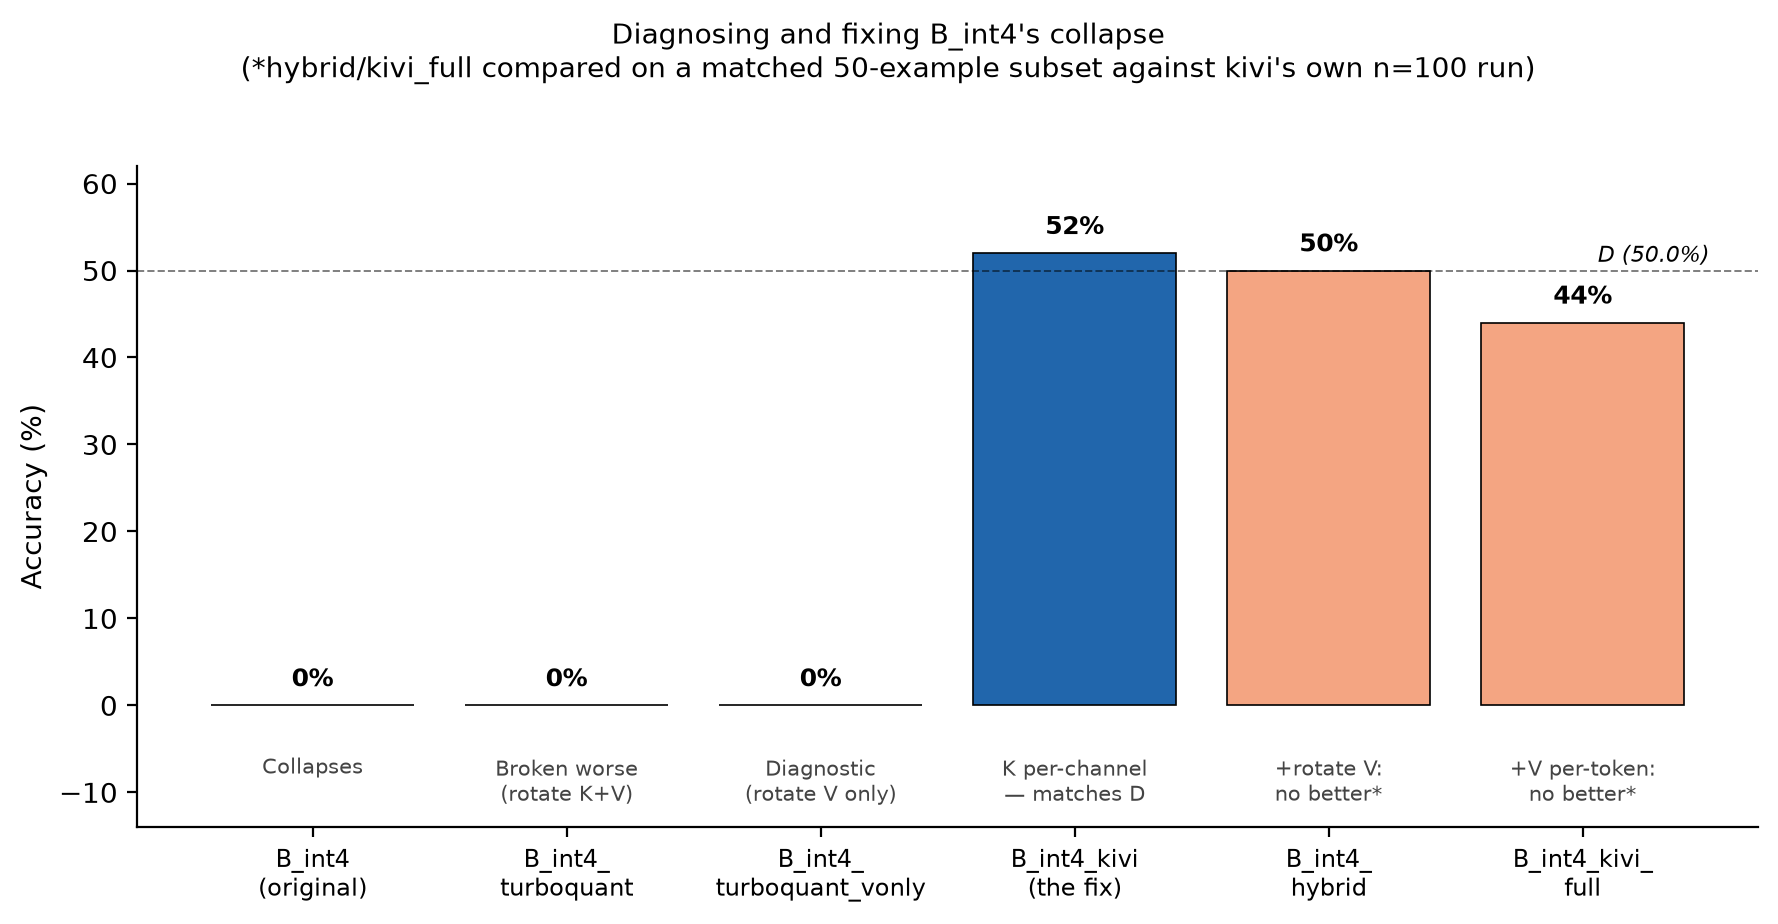
\includegraphics[width=\columnwidth]{figures/fig2_b_int4_journey.png}
\caption{The \texttt{B\_int4} diagnosis-to-fix journey: collapse, a
broken rotation-based attempt, an isolating diagnostic, the working fix
(\texttt{B\_int4\_kivi}), and two value-side variants that did not
improve on it.}
\label{fig:b_int4_journey}
\end{figure}

\paragraph{Finding 8: layer-selection's accuracy cost is architecture-
dependent.} On Mistral-7B-Instruct-v0.3 ($n=50$), dropping 9/32 layers
(28\%) cost 30.5 F1 points relative to uncompressed relay ($p=0.0001$).
On Qwen2.5-7B-Instruct ($n=100$), a near-identical proportion (8/28, 29\%)
shows a smaller, not-yet-significant cost ($p=0.34$); the cross-model
claim does not rest on that reaching significance, though, since even
Qwen's most generous uncertainty bound (F1 CI upper $+16.4$ points) is
under half of Mistral's confirmed collapse. Qwen3-8B ($n=50$) sharpens
rather than complicates this contrast: \texttt{D} numerically edges out
\texttt{A} (56.0\% versus 54.0\%), but this is noise, not a real effect,
McNemar $p=1.0$ on only 3 discordant pairs out of 50, F1 bootstrap CI
crossing zero. Read correctly, this is a second model, after Qwen2.5,
where layer-selection's cost is statistically indistinguishable from
zero, against Mistral's single confirmed, significant collapse, evidence
for architecture-dependence specifically, not for ``layer-selection is
usually costly'' or ``usually free.'' This is consistent with prior work
finding layer redundancy architecture- and protocol-dependent, not a
fixed property of a given compression ratio. Beyond this accuracy gap,
\texttt{D}'s incorrect answers also differ in character between models,
not only in rate; we summarize this briefly here and report the full
statistics, including a check we ran against an obvious decoding
confound, in Appendix~\ref{app:failurechar}.

\paragraph{Finding 9: KVCOMM-style offset correction (\texttt{E}) fails
catastrophically, independent of a decoding confound we explicitly ruled
out.} \texttt{D} versus \texttt{E}: McNemar $p\approx0.00003$, both
before and after an unrelated repetition-penalty fix that changed several
other configurations' numbers (Limitations). Manual inspection of
\texttt{E}'s raw output shows duplicated phrases and hallucinated content
inconsistent with the anchor-corrected cache carrying usable information,
not merely a lower-quality-but-coherent answer. This failure is
consistent with the pattern this subsection documents throughout: the
technique assumes a deviation observed for one question transfers to
another, an exchangeability assumption our causal findings above do not
support.

\paragraph{Finding 10: a calibration signal's own confidence does not
predict downstream layer-selection safety, and fails in the wrong
direction.} We tested the most direct available proxy for whether our
cross-architecture gap (Finding 8) reflects the model or merely our
calibration procedure: the separation between calibration-importance
scores assigned to kept (tier-1/2) versus dropped (tier-3) layers, as a
measure of how confidently the calibration ranks layers. Qwen's mean
separation is 0.491 (tier-1 0.737, tier-3 0.246); Mistral's is larger,
0.673 (tier-1 0.851, tier-3 0.178): Mistral's calibration looks more
decisive, not less, yet Mistral is the model whose accuracy collapses
harder when that ranking is acted upon. This rules out a noisier or
less-confident calibration signal for Mistral as the explanation for
Finding 8, and supports a sharper one: the calibration objective can be
equally or more internally confident while being less reliable,
undetectable from the calibration output alone. A third data point
(Qwen3-8B) trends in the same direction but is not, on its own,
statistically meaningful at $n=3$ models; we report the full correlation
only in Appendix~\ref{app:calibration} rather than presenting it as
validating evidence here.

\paragraph{Finding 11: these architecture-dependent failures differ in
kind, not only in rate.} Beyond the accuracy gap in Finding 8,
\texttt{D}'s incorrect answers on Mistral are markedly longer and include
a genuine long tail of severe failures, fluent but fabricated tangents and
degenerate repetition loops, that are essentially absent from Qwen's
failure set, which is dominated by short, close near-misses. We checked
an obvious alternative explanation, that our fixed repetition penalty
under-penalizes Mistral relative to its own tuned defaults, against each
model's published generation defaults, and found the opposite: our
setting matches Qwen's own default exactly, while Mistral's defaults
specify no repetition penalty at all, so our setting applies more
correction for Mistral, not less. The long-tail pattern persists anyway,
weakening a decoding confound as the explanation (full character-length
statistics in Appendix~\ref{app:failurechar}).

\begin{figure}[t]
\centering
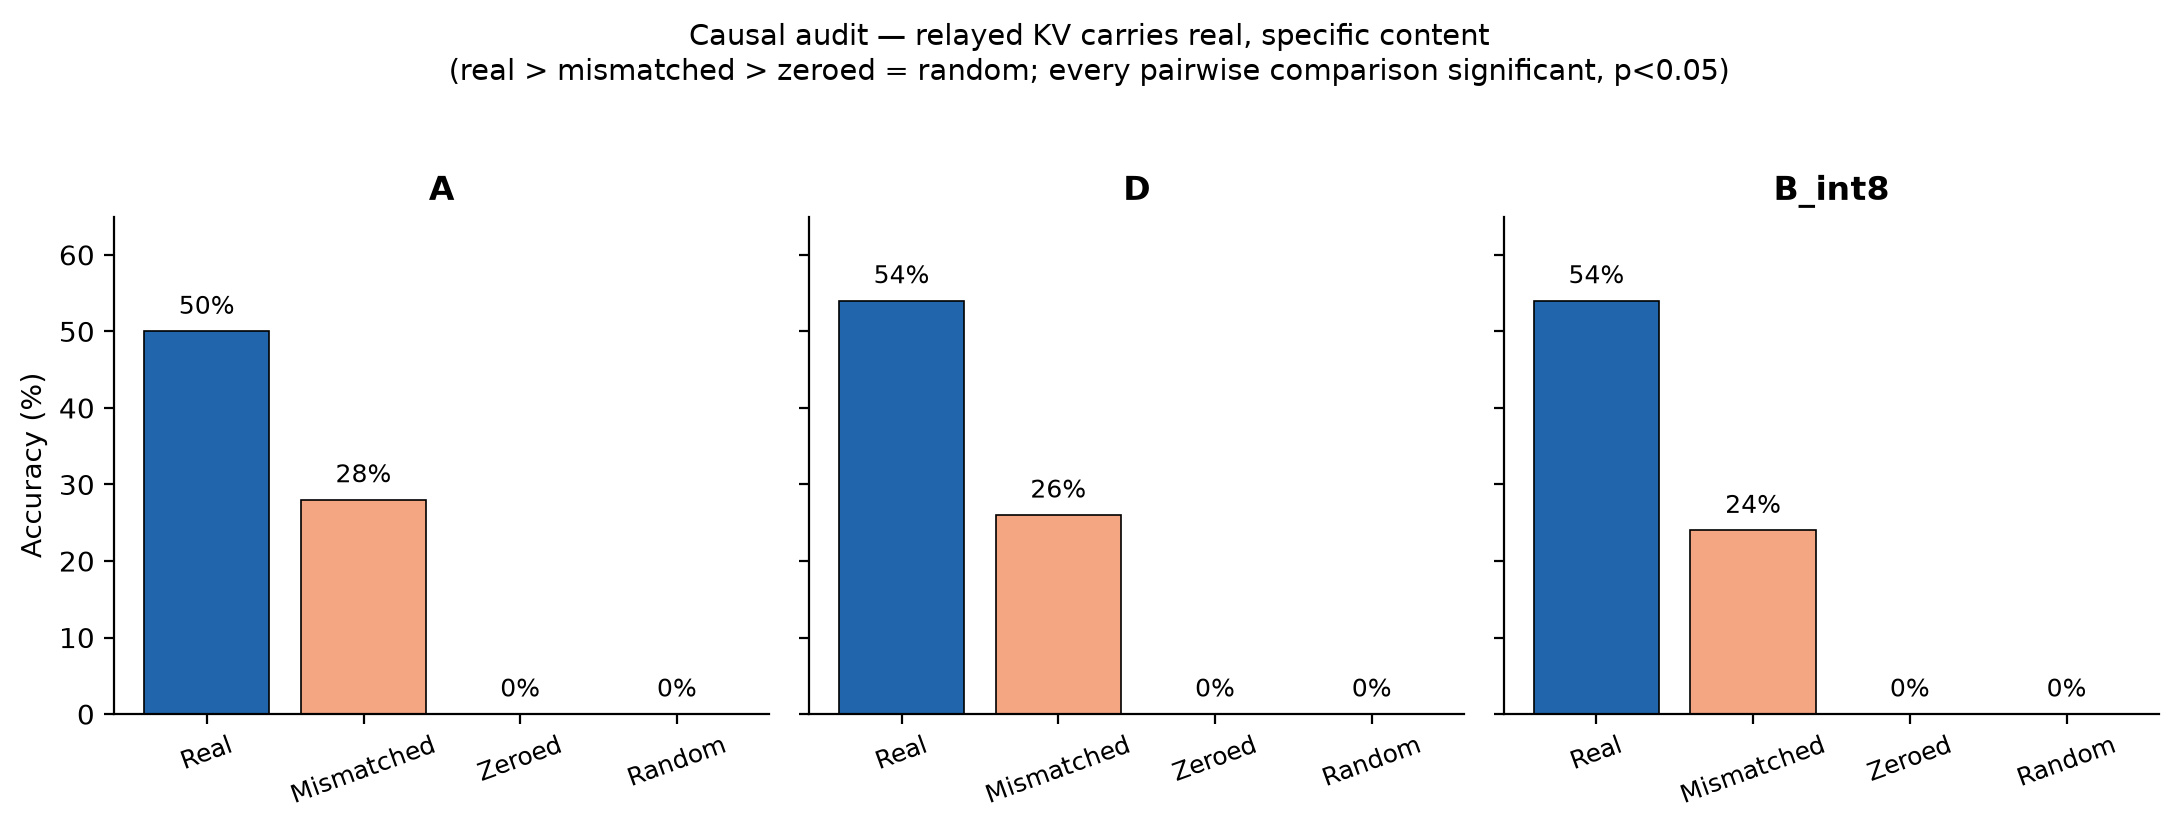
\includegraphics[width=\columnwidth]{figures/fig1_causal_audit.png}
\caption{Causal audit on the sequential chain: real $>$ mismatched $>$
zeroed $\approx$ random, replicated across \texttt{A}, \texttt{D}, and
\texttt{B\_int8}. Every pairwise comparison is statistically
significant.}
\label{fig:causal_audit}
\end{figure}

\begin{figure}[t]
\centering
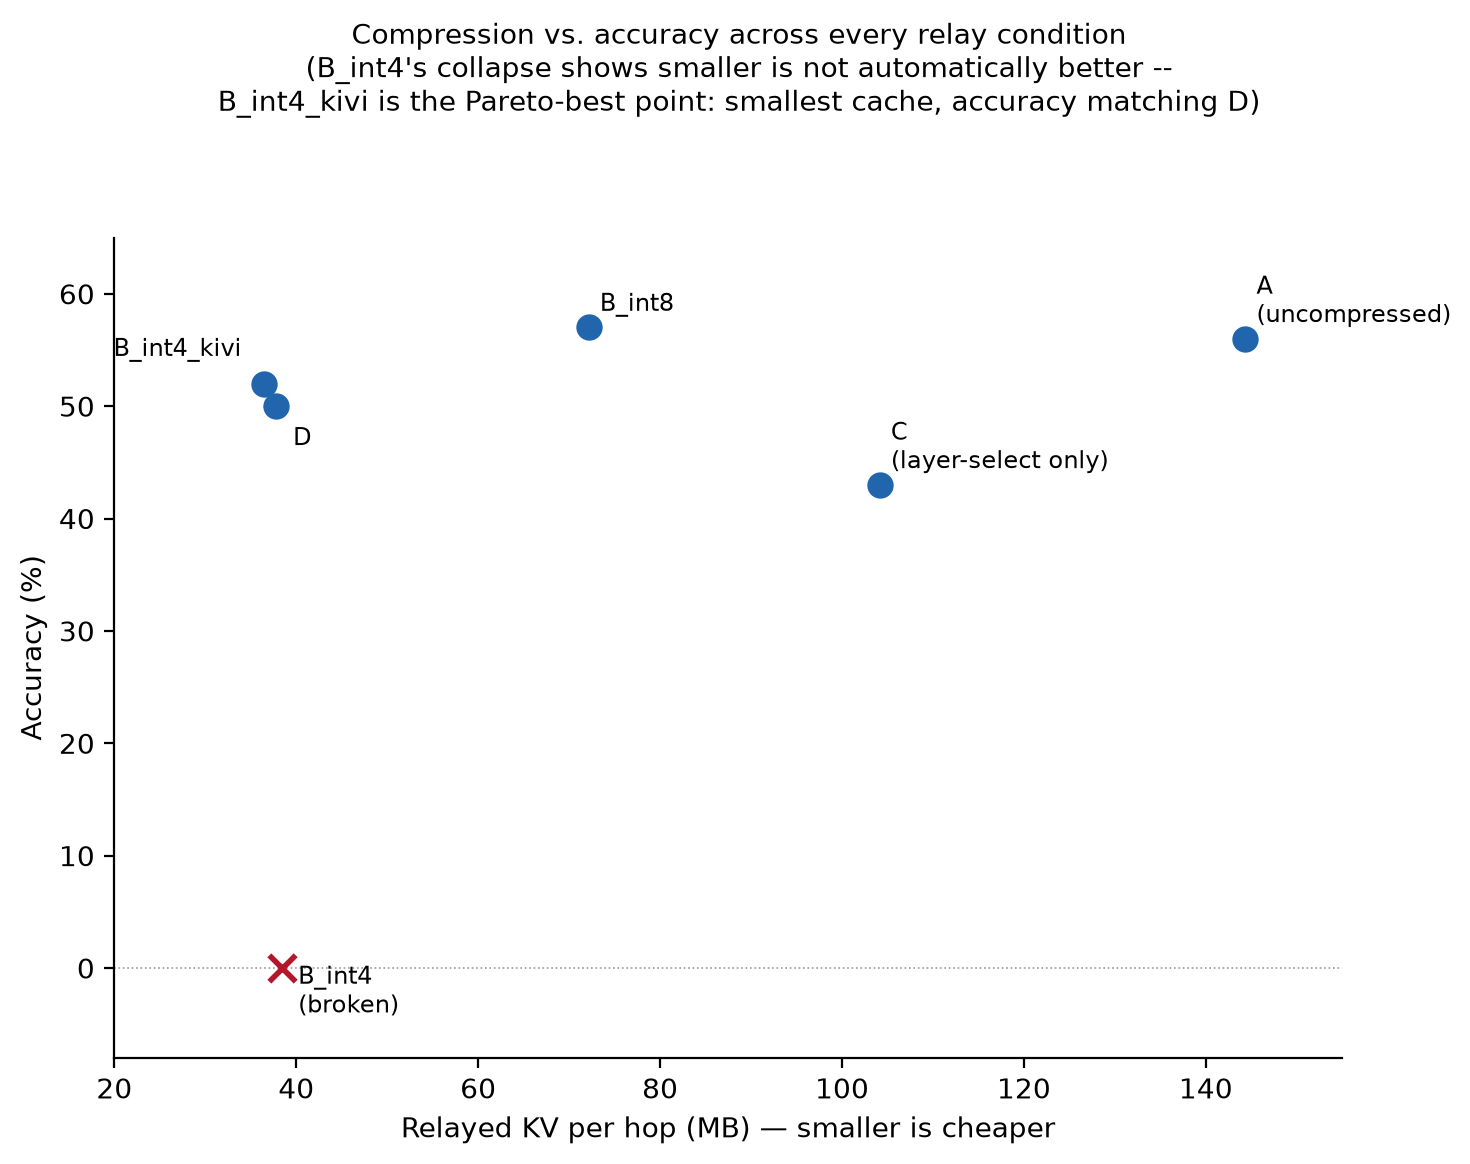
\includegraphics[width=\columnwidth]{figures/fig3_compression_pareto.png}
\caption{Compression versus accuracy across every relay condition in
Table~\ref{tab:main}. \texttt{B\_int4}'s collapse shows smaller is not
automatically better; \texttt{B\_int4\_kivi} is the Pareto-best point,
matching \texttt{D}'s accuracy at the smallest relayed cache of any
configuration tested.}
\label{fig:compression_pareto}
\end{figure}

\section{Conclusion}

Relayed KV caches should be treated as content-dependent communication
artifacts rather than interchangeable state. We establish this causally
in the simplest setting we test, a fixed sequential three-agent pipeline,
where substituting a real cache from a different question measurably and
significantly degrades downstream accuracy relative to the correct cache,
even though the substitute is just as valid a cache tensor. We then show
this ordering generalizes across topology: it holds, and gives its
cleanest demonstration, in a static fan-in decomposition, and it survives
a dynamic, model-driven delegation loop that the model constructs for
itself rather than one a system designer fixes in advance, where a
complementary behavioral signal resolves a comparison final-answer
accuracy alone could not. At the same time, the finding has a limit we
report rather than obscure: on Qwen3-8B, content-dependence itself is not
statistically distinguishable for two of our three comparisons, and a
calibration procedure's own internal confidence does not predict, and in
fact misdirects on, which architecture is safe to compress along the
depth axis. Building on this causal foundation, we show it has direct
consequences for KV-cache compression and transformation: a technique
that happens not to disturb the structure the receiver uses (uniform
8-bit quantization) is free; a technique that disrupts RoPE's position-
dependent key structure (naive 4-bit quantization, and a rotation-based
fix) fails, in one case catastrophically; a technique that respects that
structure instead (a per-channel fix) resolves the failure at genuine
compression; and a technique that assumes a deviation transfers across
unrelated content (anchor-based offset correction) fails outright. We do
not claim KV caches are universally non-exchangeable, only that, under
every model, task, and topology we tested except one, treating a relayed
cache as interchangeable rather than content-specific predicts the wrong
outcome. Systems that relay or transform KV caches between agents should
account for the fact that preserving the cache's content and structure
matters, rather than assuming that a tensor of the right shape and rough
statistics is automatically an adequate substitute.

\section*{Limitations}

\paragraph{Causal audit scope, bleed-through, and remaining topology
questions.} The causal audit now covers every relay condition in this
paper except \texttt{B\_int4} itself, which is uninformative to audit
given it already collapses unaudited (Section~\ref{sec:results}). The
bleed-through analysis (Finding 3) remains narrower: a manual review of
20 of 36 incorrect \texttt{A\_audit\_mismatched} examples by one
annotator, with no automated classifier or inter-annotator agreement
check, a qualitative, exploratory observation, not a validated rate; a
rigorous version would need an automated or multiply annotated
classification over the full set of incorrect examples, which we did not
have the budget to complete. On the recursive delegation topology
specifically, getting a working, coherent baseline required diagnosing
and fixing several real engineering failure modes, summarized briefly
here with full detail in Appendix~\ref{app:nondeterminism}; even with
those fixed, the $\texttt{kv}$-versus-$\texttt{text}$ accuracy comparison
remains genuinely unresolved at $n=50$, not merely underpowered in a way
we expect more data to resolve trivially. We report the causal-audit
result, which does resolve, as this topology's real contribution, and
leave the accuracy comparison open rather than claim more than the
evidence supports. Beyond the three topologies tested here, a genuinely
adversarial fan-in topology \citep{latentagentslie2026} and LatentMAS's
layer-wise KV concatenation \citep{latentmas2026} remain untested against
our specific causal-audit methodology; both are real, cited, not-yet-
attempted extensions, not gaps we found and left unnamed.

\paragraph{Single-process, single-GPU evaluation.} Every experiment runs
within one Python process on one RTX 4090: no \texttt{KVMessage} is ever
serialized or transmitted over a network. Compression-ratio and
transmitted-byte accounting reflects what a real distributed deployment
would need to send and is meaningful on that basis, but our latency
numbers exclude network transfer time, and smaller relayed caches are not
observed to be faster in this setup, since the model still executes every
transformer layer regardless of what its injected cache contains. As
stated in Results, a compression ratio in this paper characterizes
communication cost and accuracy tradeoffs, not a measured end-to-end
deployment speedup. This single-GPU constraint also bounded the sample
sizes and the number of model and configuration combinations we were able
to test; a systems-scale deployment study (multi-GPU, real network
transfer, throughput under concurrent load) was out of scope.

\paragraph{Statistical power and replication.} We report paired
significance tests (exact McNemar) and bootstrap confidence intervals for
every headline comparison; several, INT8's near-zero cost, offset
correction's catastrophic failure, Mistral-7B's layer-selection collapse,
are significant at conventional thresholds even at our evaluation scale.
Others are not: at $n=100$, we cannot yet statistically distinguish
Qwen2.5-7B's layer-selection condition from its uncompressed baseline in
isolation (power $\approx$15\%; roughly 3x the current sample size would
be needed). Our cross-architecture claim rests on the independently
well-powered Mistral-7B result, not the underpowered Qwen-only
comparison. Relatedly, \texttt{B\_int4\_kivi}'s comparison against
\texttt{D} (statistically indistinguishable, McNemar $p=0.86$) rests on a
single $n=100$ run each, not a multi-seed or replicated evaluation; we
report the confidence interval alongside the point estimate specifically
so ``matches \texttt{D}'' is read as the current best estimate under one
run, not a claim strengthened by replication we have not performed.

\paragraph{Scope: three models (one only partially), mostly one task,
greedy decoding.} We test Qwen2.5-7B-Instruct and Mistral-7B-Instruct-v0.3
(chosen for architectural diversity at comparable scale) on the full
suite of configurations, and Qwen3-8B on \texttt{A}/\texttt{D} only
($n=50$), specifically to extend the architecture-dependence claim and
the tier-separation correlation to a third point, not to replicate the
causal audit or compression-fix findings on a third architecture. A
fourth candidate, Phi-3.5-mini-instruct, was evaluated and dropped: after
fixing two real bugs in how our pipeline hands decode off to
\texttt{model.generate()} under non-default RoPE scaling, the model still
failed to produce coherent output once the pipeline's cumulative relayed
context crossed roughly 4{,}096 tokens, the model's
\texttt{original\_max\_position\_embeddings}. We isolated this to a
pre-existing limitation of the model and library combination itself, not
our pipeline: plain, unmodified \texttt{model.generate()}, with no relay,
injection, or pipeline code involved at all, degrades into the identical
repetition-garbage failure signature once forced past the same threshold
on a single, ordinary generation call. Since HotpotQA's per-hop contexts
(1{,}500--2{,}500+ tokens) routinely push a three-agent relay chain's
cumulative cache past this threshold, this rules Phi-3.5-mini-instruct
out for this pipeline regardless of further pipeline-side fixes. Whether
findings, particularly layer-selection's architecture-dependence, extend
to substantially larger or smaller models, mixture-of-experts
architectures, or models outside this decoder-only, grouped-query-
attention, RoPE lineage remains largely untested beyond this one
additional data point. One further methodological risk worth flagging:
Cheng et al.\ \citep{latentcommpay2026} report at least one model pairing
where the receiver could not consume a relayed cache at all, i.e.
cross-architecture relay can fail at the precondition stage, not just on
accuracy; a null result under those conditions would itself be
informative, not a bug. All of our own architecture variation is between
pipeline runs (the same model family fills every agent role within a
given run); whether a single pipeline mixing architectures across agent
roles is even viable is untested and, to our knowledge, an open problem
in this literature more broadly: KVCOMM itself flags relay between agents
with identical architectures but different weights, and agents with
different attention formulations, as work it leaves for future
exploration, and we inherit that same gap rather than closing it. Nearly
all results are on HotpotQA (distractor configuration); we ran one
$n=50$ confirmatory check on GSM8K (Qwen, \texttt{A}/\texttt{D}/full
causal audit on \texttt{A}) and both headline findings replicated
cleanly, \texttt{D} matched \texttt{A}'s accuracy exactly (McNemar
$p=1.0$, more decisively free than on HotpotQA) and the causal audit's
three-tier ordering held with every pairwise comparison significant
($p<0.0002$), larger effect sizes than the original HotpotQA run. This is
one run on one additional task family, not a systematic multi-task
study; we did not extend it to \texttt{B\_int8}/\texttt{D}-family causal
audits or Mistral, and report it as suggestive, not as evidence the
claims generalize broadly across tasks. This matters specifically for the
offset-correction negative result: KVCOMM was evaluated on MMLU, GSM8K,
and HumanEval, none of which is multi-hop QA, and whether the technique
fares differently on the more homogeneous task family it was originally
validated on remains open (our own GSM8K check did not re-test
\texttt{E}). All results additionally use greedy decoding
(\texttt{do\_sample=False}); we did not evaluate under sampling or
self-consistency, which could interact differently with a degraded or
compressed relayed context than with a full one.

\paragraph{Nibble-packing is unit-tested, not deployment-tested.} We
implement real two-values-per-byte packing for every bits==4 tensor
(Appendix~\ref{app:nibble}), verified via round-trip pack/unpack
exactness and bit-identical \texttt{compress}/\texttt{decompress} output
with and without packing on synthetic tensors. This is standalone
tensor-level testing, not an end-to-end GPU rerun with the new packing
path in the live pipeline; accuracy and F1 are unaffected in principle
(packing changes storage format, not values, and the unit tests confirm
this directly), but we have not re-run the full $n=100$ HotpotQA
evaluation with packing enabled to confirm no integration issue exists
between the compressor and the rest of the pipeline (cache
reconstruction, device placement, batch handling). The reported accuracy
numbers throughout this paper come from pre-packing runs; only the
compression-ratio figures reflect the packing-enabled compressor.

\paragraph{Partial reproduction of adapted and considered techniques.}
Our rotation-based quantization covers PolarQuant's core rotate-then-
quantize mechanism but omits TurboQuant's QJL bias-correction term; our
KIVI-inspired fix omits the original method's group-wise windowing and
fp16 residual buffer, implementing full-sequence per-channel quantization
only, the minimal change isolating the RoPE-interaction mechanism we
diagnosed, not a complete reproduction. We report both as inspired-by
implementations scoped to test a specific hypothesis, not certified
reproductions, and encourage readers wanting the original techniques'
full guarantees to consult the primary sources. We considered but did not
implement a fourth layer-reconstruction strategy, Orthogonal Backfill
\citep{orthobackfill2026}: its published formula requires attention
weights this pipeline's \texttt{sdpa} decode path does not expose, and
given our own evidence that naive or simplified reproductions can
actively mislead (the rotation-based quantization finding above), we
chose not to ship an approximated version under time pressure, a scoping
decision, not a result.

We checked ARR's guidance before deciding whether a separate Ethical
Considerations section was warranted: this work uses two long-established
public benchmarks (HotpotQA, GSM8K), two openly released model
checkpoints, no human subjects, no crowdsourcing, and no new data
collection; we are not aware of a concern specific to this paper beyond
what this section already covers.

\bibliography{references_rlm_focus}
\bibliographystyle{acl_natbib}

\appendix

\section{Implementation and verification detail}

This appendix collects implementation and debugging detail referenced
from the main text, kept out of the body for length but preserved here
in full since each documents a real, verified finding rather than an
assumption.

\subsection{Rotation-based quantization: full diagnostic detail}
\label{app:rotation}

The rotation-based quantization scheme described in Related Work and
Finding 7 produced, on a real model run, severely out-of-distribution
decoded tokens: literal fragments such as \texttt{.HttpServletResponse}
and isolated CJK characters unrelated to the input language, a failure
shape inconsistent with ordinary quantization noise. The isolating
ablation (rotating only V, leaving K on the exact same code path as plain
\texttt{B\_int4}, verified bit-identical via unit test) reverted this to
ordinary \texttt{B\_int4}-style degenerate repetition output (for
example, repeated tokens such as ``2 2 2 2'' or ``0 0 0 0''), confirming
the bizarre failure mode was specific to rotating K, not an artifact of
4-bit precision in general.

\subsection{RLM+KV non-determinism: diagnosis and fix}
\label{app:nondeterminism}

An earlier run of the recursive, model-driven delegation experiment
(Finding 5) was not run-to-run deterministic. Diffing raw generations for
the identical 50 questions between two independent runs under greedy
decoding (\texttt{do\_sample=False}), same model, same questions,
confirmed via literal string comparison rather than assumed from a
summary statistic, found that 15 of 50 (30\%) \texttt{text}-channel
examples produced genuinely different output. Unlike the two fixed
topologies in this paper, which are confirmed bit-identical across
reruns, this REPL-based prototype's long, many-turn, self-referential
decoding loop is evidently sensitive to GPU floating-point non-
associativity: a small numerical difference at one argmax decision can
cascade through a multi-turn trajectory, particularly since each turn
involves the model writing and executing its own code, where small
wording shifts change what actually runs.

We fixed this by forcing \texttt{torch.use\_deterministic\_algorithms
(True, warn\_only=True)} and setting \texttt{CUBLAS\_WORKSPACE\_CONFIG}
before any CUDA context exists (before \texttt{torch} is imported). We
verified the fix directly rather than assume it worked: a rerun of the
\texttt{text} channel on 20 questions produced 0/20 differing raw
answers against the pre-fix run, including all 7 of the examples that
were part of the original 15/50 divergent set. We then reran the full
five-channel, $n=50$ ladder independently and diffed every field, not
only the ones reported in Finding 5: exact match, F1, timeout rate, and
delegation-call count are bit-identical across both runs (0 of 250 raw
answers differ across all five conditions). One narrow, harmless nuance
surfaced only by diffing every field: 33 of the \texttt{random}
condition's 50 examples show different intermediate turn-by-turn wording
between the two runs, even though both independently exhaust their turn
budget on the identical question with the identical final outcome
(timeout, no answer, identical delegation-call count); this never affects
any scored quantity reported in this paper. The results reported in
Finding 5 are confirmed reproducible under this fix, not a single sample
from an uncontrolled process.

Separately from this non-determinism fix, getting a working, coherent
baseline for this topology at all required diagnosing and fixing three
real engineering failure modes: a sub-call's own prompt framing leaking
into the receiver's attention when spliced without isolating the
generated answer span; a session-wide repetition-tracking loss specific
to a persistent, turn-continuing cache; and a RoPE position-shift bug
specific to splicing an answer-only, prompt-truncated child KV, whose fix
we verified two ways, a corrected unit test and a real-model rerun
showing every previously degenerate example become coherent.

\subsection{Fan-in causal audit: an early design bug and its fix}
\label{app:faninbug}

An early version of the fan-in causal audit (Finding 4) substituted only
one of the two children's KV by default, leaving the other child's real
content available to the aggregator as an unaudited shortcut. This
initially produced a near-null result (3/10 exact-match for the real
condition versus 3/10 for the zeroed condition at a small pilot scale)
that, on inspection of raw predictions, turned out to be a weaker test
than intended rather than a genuine null: 5 of the 10 zeroed-condition
outputs already showed the expected garbled-output signature, meaning the
aggregator was still succeeding on the other, uncorrupted child often
enough to mask the effect. We fixed this by adding a mode that
substitutes every child's KV rather than a single one (extracted into a
directly testable helper function with its own unit tests), matching the
full-relay-corruption strength of the sequential pipeline's own audit.
The corrected result is the one reported in Finding 4.

\subsection{Nibble-packing: byte-accounting bug and real fix}
\label{app:nibble}

Our compressor initially stored every quantized tensor as one full
\texttt{torch.uint8} per element regardless of bit-width: no nibble-
packing existed anywhere in the implementation, so a 4-bit value took the
same byte an 8-bit value did. Our first-reported compression ratios
assumed packing that did not exist, overstating 4-bit configurations'
real compression. We implemented genuine two-values-per-byte packing
(pack after quantizing for bits==4, unpack before dequantizing) and
verified it with unit tests covering round-trip pack and unpack
exactness, including odd-length and padding edge cases, full-nibble-range
coverage, and, most directly relevant, bit-identical
\texttt{compress}/\texttt{decompress} output with and without packing
enabled, confirming packing is a pure storage-format change with no
effect on dequantized values. The corrected, packing-backed compression
ratios reported in Table~\ref{tab:main} and throughout this paper land
back at almost exactly the originally reported figures, not a
coincidence: the original formula's arithmetic (0.5 bytes per element for
4-bit) was always what real packing would produce; the bug was that
nothing in the compressor actually packed anything.

\subsection{Calibration tier-separation correlation across three models}
\label{app:calibration}

Finding 10 reports that calibration confidence (the separation between
kept- and dropped-layer importance scores) does not predict layer-
selection safety on two models, Qwen2.5-7B-Instruct (separation 0.491)
and Mistral-7B-Instruct-v0.3 (separation 0.673), and fails in the wrong
direction. Adding Qwen3-8B as a third point (separation 0.591, between
the other two, pairing with \texttt{D}'s near-zero accuracy cost on this
model from Finding 8) lets us compute a correlation between tier
separation and degradation across the three models: Pearson $r=0.619$,
Spearman $r=0.500$. We report this only as a trend consistent with the
two-model finding, not as validating evidence. With $n=3$ models, this
correlation is barely more informative than the $n=2$ qualitative
comparison it extends, and we would not cite it as meaningful without at
least two or three further model families, which we did not have the
resources to add to this draft.

\subsection{Layer-selection failure character: full statistics}
\label{app:failurechar}

Finding 11 reports that \texttt{D}'s incorrect answers differ in
character, not only in rate, between Qwen2.5-7B-Instruct and Mistral-7B-
Instruct-v0.3. In full: Qwen's incorrect answers average 18 characters,
with 2\% exceeding 150 characters, overwhelmingly close, traceable near-
misses (reformatted dates, dropped honorifics, single-character typos).
Mistral's average 109 characters, with 15\% exceeding 150 characters and
a maximum of 1,454, and include fluent fabricated tangents (for example,
a full invented biography of a person unrelated to the question) and
degenerate repetition loops, failure modes essentially absent from
Qwen's failure set. We checked the most obvious confound before trusting
this difference: whether our uniform \texttt{repetition\_penalty=1.05}
under-penalizes Mistral relative to its own tuned decoding defaults. We
checked both models' published \texttt{generation\_config.json} directly:
Qwen's own default is exactly 1.05, while Mistral's specifies no
repetition penalty at all, meaning our setting applies more correction
for Mistral than its own baseline calls for, the opposite of what the
confound would need to explain the pattern. The long-tail failure pattern
persists regardless, weakening rather than supporting a decoding-
hyperparameter explanation.

\end{document}
